\item \textbf{{[}JPJC/PRELIM/9597/2019/P2/Q4{]} }

Object-oriented programming is used to store and process data for
a company\textquoteright s payroll. 
\begin{center}
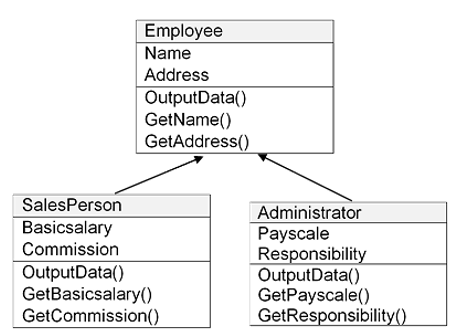
\includegraphics[width=0.5\paperwidth]{C:/Users/Admin/Desktop/Github/question_bank/LyX/static/img/9597-JPJC-2019-P2-Q4-1}
\par\end{center}
\begin{enumerate}
\item With reference to the class diagram shown above, explain: 
\begin{enumerate}
\item data encapsulation, and how classes support information hiding and
implementation independence. \hfill{}{[}3{]}
\item inheritance, and how it promotes software reusability. \hfill{}{[}2{]}
\end{enumerate}
\end{enumerate}